\documentclass[a4paper]{article}
\usepackage{longtable,float,hyperref,color,amsmath,amsxtra,amssymb,latexsym,amscd,amsthm,amsfonts,graphicx}
\numberwithin{equation}{section}
\allowdisplaybreaks
\usepackage{fancyhdr}
\pagestyle{fancy}
\fancyhf{}
\fancyhead[RE,LO]{\footnotesize \textsc \leftmark}
\cfoot{\thepage}
\renewcommand{\headrulewidth}{0.5pt}
\setcounter{tocdepth}{3}
\setcounter{secnumdepth}{3}
\usepackage{imakeidx}
\makeindex[columns=2, title=Alphabetical Index, 
           options= -s index.ist]
\title{\huge Differential Geometry Assignment 002}
\author{\textsc{Nguyen Quan Ba Hong}\\
{\small Students at Faculty of Math and Computer Science,}\\ 
{\small Ho Chi Minh University of Science, Vietnam} \\
{\small \texttt{email. nguyenquanbahong@gmail.com}}\\
{\small \texttt{blog. \url{www.nguyenquanbahong.com}} 
\footnote{Copyright \copyright\ 2016-2017 by Nguyen Quan Ba Hong, Student at Ho Chi Minh University of Science, Vietnam. This document may be copied freely for the purposes of education and non-commercial research. Visit my site \texttt{\url{www.nguyenquanbahong.com}} to get more.}}}
\begin{document}
\maketitle
\begin{abstract}
This assignment aims at solving \textbf{Exercises 5, 6, 7}, p.168-169, \cite{1}.
\end{abstract}
\newpage
\tableofcontents
\newpage
\listoffigures
\newpage
\section{Problems}
\textbf{Problem 1 (Exercise 5, p.168, \cite{1}).} \textit{Consider the parametrized surface (Enneper's surface)}
\begin{align}
\mathbf{x} \left( {u,v} \right) = \left( {u - \frac{{{u^3}}}{3} + u{v^2},v - \frac{{{v^3}}}{3} + v{u^2},{u^2} - {v^2}} \right),
\end{align}
\textit{and show that}
\begin{enumerate}
\item \textit{The coefficients of the first fundamental form are}
\begin{align}
\label{1.2}
E = G = {\left( {1 + {u^2} + {v^2}} \right)^2},F = 0.
\end{align}
\item \textit{The coefficients of the second fundamental form are}
\begin{align}
\label{1.3}
e = 2,g =  - 2,f = 0.
\end{align}
\item \textit{The principal curvatures are}
\begin{align}
\label{1.4}
{k_1} = \frac{2}{{{{\left( {1 + {u^2} + {v^2}} \right)}^2}}},{k_2} =  - \frac{2}{{{{\left( {1 + {u^2} + {v^2}} \right)}^2}}}.
\end{align}
\item \textit{The lines of curvature are the coordinate curves.}
\item \textit{The asymptotic curves are $u+v =\mbox{const.}$, $u-v=\mbox{const}$.}
\end{enumerate}
\textsc{Solution.} 
\begin{enumerate}
\item To obtain the first fundamental form, we compute 
\begin{align}
\label{1.5}
{\mathbf{x}_u} &= \left( {1 - {u^2} + {v^2},2uv,2u} \right),\\
{\mathbf{x}_v} &= \left( {2uv,1 - {v^2} + {u^2}, - 2v} \right), \label{1.6}
\end{align}
and therefore 
\begin{align}
E &= \left\langle {{\mathbf{x}_u},{\mathbf{x}_u}} \right\rangle \\
 &= {\left( {1 - {u^2} + {v^2}} \right)^2} + 4{u^2}{v^2} + 4{u^2}\\
& = {\left( {1 + {u^2} + {v^2}} \right)^2},\\
F &= \left\langle {{\mathbf{x}_u},{\mathbf{x}_v}} \right\rangle \\
 &= 2uv\left( {1 - {u^2} + {v^2}} \right) + 2uv\left( {1 - {v^2} + {u^2}} \right) - 4uv\\
 &= 0,\\
G &= \left\langle {{\mathbf{x}_v},{\mathbf{x}_v}} \right\rangle \\
 &= 4{u^2}{v^2} + {\left( {1 - {v^2} + {u^2}} \right)^2} + 4{v^2}\\
 &= {\left( {1 + {u^2} + {v^2}} \right)^2},
\end{align}
i.e., \eqref{1.2} holds.
\item For the computation of the coefficients $e,g,f$ of the second fundamental form, we need to know $\mathbf{x}_u, \mathbf{x}_v$ (given by \eqref{1.5}-\eqref{1.6}), $N$, $\mathbf{x}_{uu}, \mathbf{x}_{uv}$ and  $\mathbf{x}_{vv}$:
\begin{align}
{\mathbf{x}_{uu}} &= \left( { - 2u,2v,2} \right),\\
{\mathbf{x}_{uv}} &= \left( {2v,2u,0} \right),\\
{\mathbf{x}_{vv}} &= \left( {2u, - 2v, - 2} \right).
\end{align}
Hence, 
\begin{align}
e &= \left\langle {N,{\mathbf{x}_{uu}}} \right\rangle \\
 &= \left\langle {\frac{{{\mathbf{x}_u} \wedge {\mathbf{x}_v}}}{{\left| {{\mathbf{x}_u} \wedge {\mathbf{x}_v}} \right|}},{\mathbf{x}_{uu}}} \right\rangle \\
 &= \frac{{\left( {{\mathbf{x}_u},{\mathbf{x}_v},{\mathbf{x}_{uu}}} \right)}}{{\sqrt {EG - {F^2}} }}\\
& = \frac{{\left| {\begin{array}{*{20}{c}}
{1 - {u^2} + {v^2}}&{2uv}&{ - 2u}\\
{2uv}&{1 - {v^2} + {u^2}}&{2v}\\
{2u}&{ - 2v}&2
\end{array}} \right|}}{{{{\left( {1 + {u^2} + {v^2}} \right)}^2}}}\\
& = \frac{{2{{\left( {1 + {u^2} + {v^2}} \right)}^2}}}{{{{\left( {1 + {u^2} + {v^2}} \right)}^2}}}\\
& = 2,\\
f &= \left\langle {N,{\mathbf{x}_{uv}}} \right\rangle \\
& = \frac{{\left( {{\mathbf{x}_u},{\mathbf{x}_v},{\mathbf{x}_{uv}}} \right)}}{{\sqrt {EG - {F^2}} }}\\
& = \frac{{\left| {\begin{array}{*{20}{c}}
{1 - {u^2} + {v^2}}&{2uv}&{2v}\\
{2uv}&{1 - {v^2} + {u^2}}&{2u}\\
{2u}&{ - 2v}&0
\end{array}} \right|}}{{{{\left( {1 + {u^2} + {v^2}} \right)}^2}}}\\
 &= 0,\\
g &= \left\langle {N,{\mathbf{x}_{vv}}} \right\rangle \\
& = \frac{{\left( {{\mathbf{x}_u},{\mathbf{x}_v},{\mathbf{x}_{vv}}} \right)}}{{\sqrt {EG - {F^2}} }}\\
& = \frac{{\left| {\begin{array}{*{20}{c}}
{1 - {u^2} + {v^2}}&{2uv}&{2u}\\
{2uv}&{1 - {v^2} + {u^2}}&{ - 2v}\\
{2u}&{ - 2v}&{ - 2}
\end{array}} \right|}}{{{{\left( {1 + {u^2} + {v^2}} \right)}^2}}}\\
& =  - \frac{{2{{\left( {1 + {u^2} + {v^2}} \right)}^2}}}{{{{\left( {1 + {u^2} + {v^2}} \right)}^2}}}\\
& =  - 2,
\end{align}
i.e., \eqref{1.3} holds. 
\item We recall that the principal curvatures $k_1,k_2$ are the roots of the following quadratic equation 
\begin{align}
\label{1.34}
{k^2} - 2Hk + K = 0.
\end{align}
Hence, to obtain $k_1,k_2$, it suffices to compute the Gaussian curvature $K$ and the mean curvature $H$:
\begin{align}
K &= \frac{{eg - {f^2}}}{{EG - {F^2}}}\\
 &=  - \frac{4}{{{{\left( {1 + {u^2} + {v^2}} \right)}^4}}},\\
H &= \frac{1}{2} \cdot \frac{{eG - 2fF + gE}}{{EG - {F^2}}}\\
 &= \frac{{G - E}}{{{{\left( {1 + {u^2} + {v^2}} \right)}^4}}}\\
 &= 0.
\end{align}
The quadratic equation \eqref{1.34} then becomes
\begin{align}
{k^2} -  \frac{4}{{{{\left( {1 + {u^2} + {v^2}} \right)}^4}}} = 0,
\end{align}
i.e., \eqref{1.4} holds. 
\item We directly apply the following result, which is established in p.161, \cite{1}: ``\textit{A necessary and sufficient condition for the coordinate curves of a parametrization to be lines of curvature in a neighborhood of a nonumbilical points is that $F=f=0$.}'' to Enneper's surface. It should be noted that all the points of this surface are nonumbilical since $k_1 \ne k_2$.
\item We recall that a connected regular curve $C$ in the coordinate neighborhood of $\mathbf{x}$ is an asymptotic curve if and only if for any parametrization $\alpha \left(t\right)=\mathbf{x}\left(u\left(t\right),v\left(t\right)\right)$, $t\in I$, of $C$ we have $II \left(\alpha '\left(t\right)\right) =0$, for all $t\in I$, that is, if and only if
\begin{align}
\label{1.41}
e{\left( {u'} \right)^2} + 2fu'v' + g{\left( {v'} \right)^2} = 0,\hspace{0.2cm} t \in I.
\end{align}

The differential equation of asymptotic curves \eqref{1.41}, in our situation, becomes (globally)
\begin{align}
\label{1.42}
2{\left( {u'} \right)^2} - 2{\left( {v'} \right)^2} = 0.
\end{align}
Hence, $u' + v' = 0$ or $u' - v' = 0$ satisfy \eqref{1.42}. By integrating these equations with respect to variable $t$, we conclude that the asymptotic curves are $u+v=\mbox{const.}$, and $u-v=\mbox{const}$.\hfill $\square$
\end{enumerate}
\vspace{0.5cm}
\textbf{Problem 2 (Exercise 6, p.168-169, \cite{1}).} 

\textit{(A Surface with $K \equiv  - 1$; the Pseudosphere.)} 
\begin{enumerate}
\item \textit{Determine an equation for the plane curve $C$, which is such that the segment of the tangent line between the point of tangency and some line $r$ in the plane, which does not meet the curve, is constantly equal to 1 (this curve is called the \textbf{tractrix}); see Fig. \ref{1}.}
\begin{figure}[H]
\label{1}
\centering
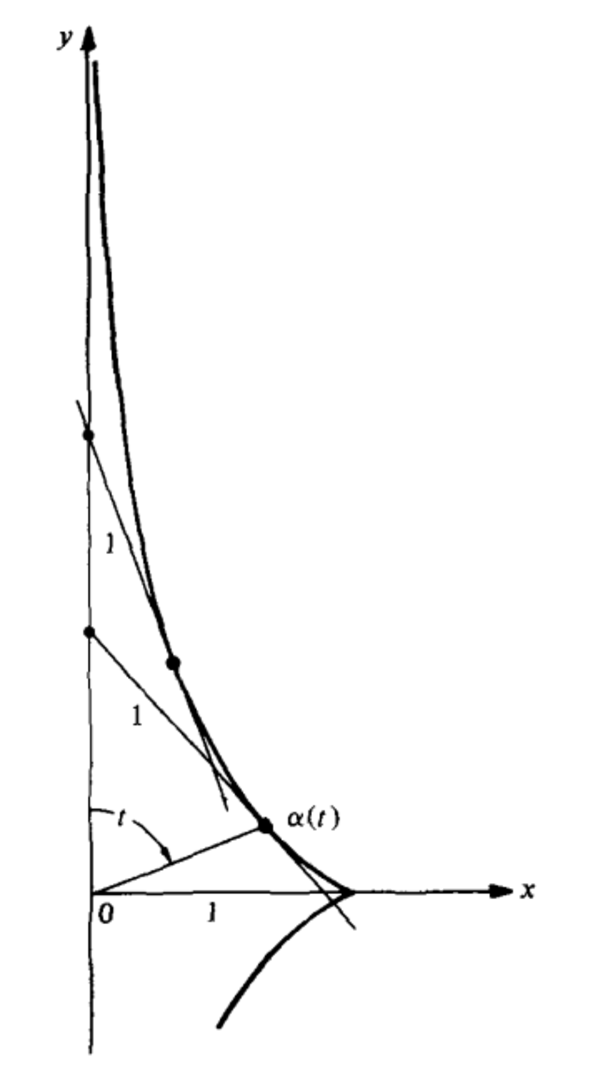
\includegraphics[scale=0.5]{1}
\caption{\textsc{The tractrix.}}
\end{figure}
\item \textit{Rotate the tractrix $C$ about the line $r$; determine if the ``surface'' of revolution thus obtained (the \textit{pseudosphere}; see Fig. \ref{2}) is regular and find out a parametrization in a neighborhood of a regular point.}
\begin{figure}[H]
\label{2}
\centering
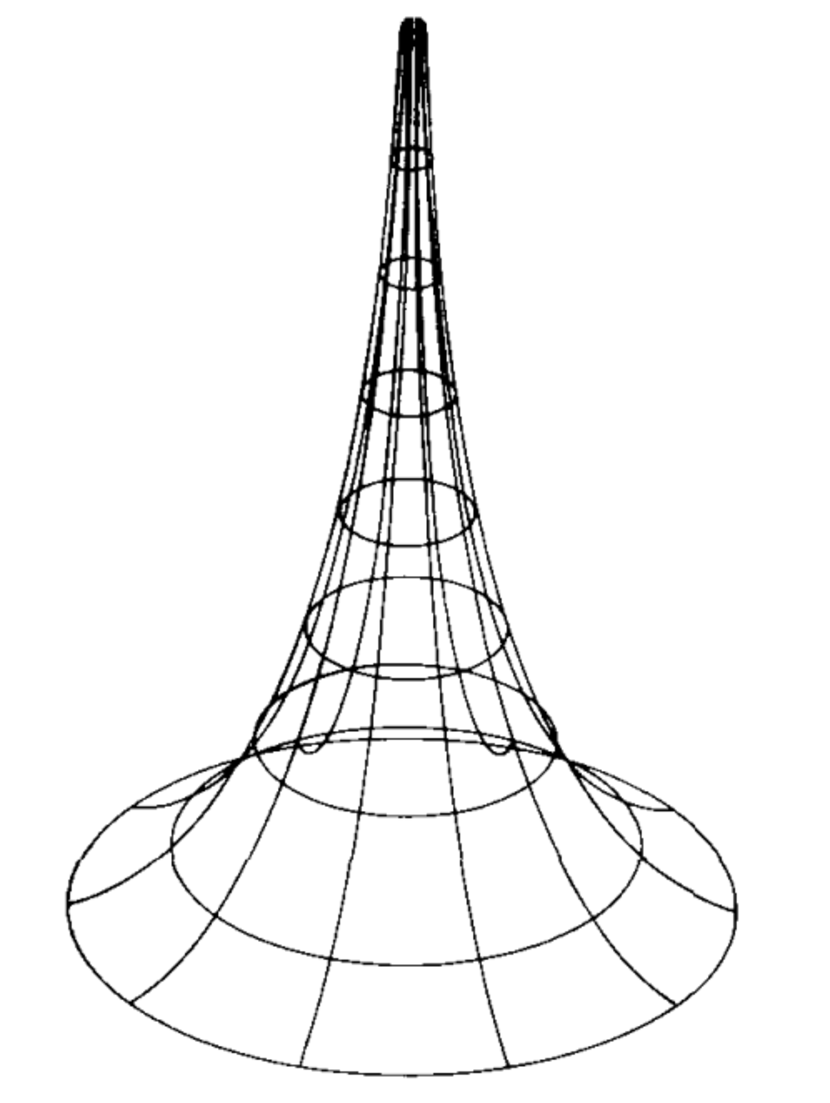
\includegraphics[scale=0.43]{2}
\caption{\textsc{The pseudosphere.}}
\end{figure}
\item \textit{Show that the Gaussian curvature of any regular point of the pseudosphere is $-1$.}
\end{enumerate}
\textsc{Solution.} 
\begin{enumerate}
\item By taking the line $r$ as the $z$ axis and a normal to $r$ as the $x$ axis, we have that
\begin{align}
\label{1.43}
z' = \frac{{\sqrt {1 - {x^2}} }}{x}.
\end{align}
By setting $x= \sin \theta$, we obtain
\begin{align}
z\left( \theta  \right) &= \int {\frac{{{{\cos }^2}\theta }}{{\sin \theta }}d\theta } \\
 &= \ln \tan \frac{\theta }{2} + \cos \theta  + C.
\end{align}
If $z\left(\frac{\pi}{2}\right) =0$, then $C=0$.
\item With the above notations; see p.76, \cite{1},
\begin{align}
x = \sin \theta ,z = \ln \tan \frac{\theta }{2} + \cos \theta ,\hspace{0.2cm}0 < \theta  < \pi ,
\end{align}
is a parametrization for the tractrix $C$ and denote by $\delta $ the rotation angle about the $z$ axis. Thus, we obtain a map
\begin{align}
\label{1.47}
\mathbf{x} \left( {\theta ,\delta } \right) = \left( {\sin \theta \cos \delta ,\sin \theta \sin \delta ,\ln \tan \frac{\theta }{2} + \cos \theta } \right),
\end{align}
from the open set $U = \left\{ {\left( {\theta ,\delta } \right) \in {\mathbb{R}^2};0 < \theta  < \pi ,0 < \delta  < 2\pi } \right\}$  into the pseudosphere $S$. 

To show that $S$ is regular, we need to prove that $\mathbf{x}$ is a parametrization of $S$, i.e., we must check condition 1, 2, and 3 of Def. 1, Sec. 2.2, p.52, \cite{1}. 
\begin{enumerate}
\item \textit{$\mathbf{x}$ is differentiable.} This is obvious by \eqref{1.47}. We write 
\begin{align}
\mathbf{x} \left( {\theta ,\delta } \right) = \left( {x\left( {\theta ,\delta } \right),y\left( {\theta ,\delta } \right),z\left( {\theta ,\delta } \right)} \right), \hspace{0.2cm} \left( {\theta ,\delta } \right) \in U,
\end{align}
where 
\begin{align}
x\left( {\theta ,\delta } \right) &= \sin \theta \cos \delta ,\\
y\left( {\theta ,\delta } \right) &= \sin \theta \sin \delta ,\\
z\left( {\theta ,\delta } \right) &= \ln \tan \frac{\theta }{2} + \cos \theta ,
\end{align}
have continuous partial derivatives of all orders in $U$.
\item \textit{$\mathbf{x}$ is a homeomorphism.} To show that $\mathbf{x}$ is a homeomorphism, we first show that $\mathbf{x}$ is one-to-one. In face, since $\left( {\sin \theta ,\ln \tan \frac{\theta }{2} + \cos \theta } \right)$ is a parametrization of $C$, given $z$ and ${x^2} + {y^2} = {\sin ^2}\theta $, we can determine $\theta$ uniquely. Thus, $\mathbf{x}$ is one-to-one. 

We remark that because $\left( {\sin \theta ,\ln \tan \frac{\theta }{2} + \cos \theta } \right)$ is a parametrization of $C$, $\theta$ is a continuous function of $z$ and of $\sqrt {{x^2} + {y^2}}$ and thus a continuous function of $\left(x,y,z\right)$. \footnote{Indeed, $\theta$ can be represented as
\begin{align}
\theta  &= {\left( {\ln  \circ \tan  \circ f + \cos } \right)^{ - 1}}\left( z \right),\\
\theta  &= \arcsin \sqrt {{x^2} + {y^2}} ,
\end{align}
where $f:\theta \mapsto \frac{\theta}{2}$.}

To prove that $\mathbf{x}^{-1}$ is continuous, it remains to show that $\theta$ is a continuous function of $\left(x,y,z\right)$. To see this, we first observe that if $\theta \ne \pi$, we obtain, since $\sin \theta  \ne 0$ ($0 <\theta <\pi$),
\begin{align}
\tan \frac{\delta }{2} &= \frac{{\sin \frac{\delta }{2}}}{{\cos \frac{\delta }{2}}}\\
& = \frac{{2\sin \frac{\delta }{2}\cos \frac{\delta }{2}}}{{2{{\cos }^2}\frac{\delta }{2}}}\\
& = \frac{{\sin \delta }}{{1 + \cos \delta }}\\
& = \frac{{\frac{y}{{\sin \theta }}}}{{1 + \frac{x}{{\sin \theta }}}}\\
 &= \frac{y}{{x + \sqrt {{x^2} + {y^2}} }},
\end{align}
hence,
\begin{align}
\delta  = 2{\tan ^{ - 1}}\frac{y}{{x + \sqrt {{x^2} + {y^2}} }}.
\end{align}
Thus, if $\delta \ne \pi$, $\delta$ is a continuous function of $\left(x,y,z\right)$. By the same token, if $\delta$ is in a small interval about $\pi$, we obtain
\begin{align}
\delta  = 2{\cot ^{ - 1}}\frac{y}{{ - x + \sqrt {{x^2} + {y^2}} }}.
\end{align}

Thus, $\delta$ is a continuous of $\left(x,y,z\right)$. This shows that $\mathbf{x}^{-1}$ is continuous. 
\item \textit{The regularity condition.} We will prove that for each $q \in U$, the differential $d\mathbf{x}_q: \mathbb{R}^2 \to \mathbb{R}^3$ is one-to-one. To this end, we consider the following Jacobian determinants
\begin{align}
\frac{{\partial \left( {x,y} \right)}}{{\partial \left( {\theta ,\delta } \right)}} &= \left| {\begin{array}{*{20}{c}}
{{x_\theta }}&{{x_\delta }}\\
{{y_\theta }}&{{y_\delta }}
\end{array}} \right|\\
& = \left| {\begin{array}{*{20}{c}}
{\cos \theta \cos \delta }&{ - \sin \theta \sin \delta }\\
{\cos \theta \sin \delta }&{\sin \theta \cos \delta }
\end{array}} \right|\\
& = \sin \theta \cos \theta {\cos ^2}\delta  + \sin \theta \cos \theta {\sin ^2}\delta \\
& = \sin \theta \cos \theta ,
\end{align}
which is nonzero for $\theta  \ne \frac{\pi }{2}$,
\begin{align}
\frac{{\partial \left( {y,z} \right)}}{{\partial \left( {\theta ,\delta } \right)}} &= \left| {\begin{array}{*{20}{c}}
{{y_\theta }}&{{y_\delta }}\\
{{z_\theta }}&{{z_\delta }}
\end{array}} \right|\\
& = \left| {\begin{array}{*{20}{c}}
{\cos \theta \sin \delta }&{\sin \theta \cos \delta }\\
{\dfrac{1}{{\sin \theta }}}&0
\end{array}} \right|\\
& =  - \cos \delta ,
\end{align}
which is nonzero for $\delta  \notin \left\{ {\frac{\pi }{2},\frac{{3\pi }}{2}} \right\}$, and 
\begin{align}
\frac{{\partial \left( {x,z} \right)}}{{\partial \left( {\theta ,\delta } \right)}} &= \left| {\begin{array}{*{20}{c}}
{{x_\theta }}&{{x_\delta }}\\
{{z_\theta }}&{{z_\delta }}
\end{array}} \right|\\
& = \left| {\begin{array}{*{20}{c}}
{\cos \theta \cos \delta }&{ - \sin \theta \sin \delta }\\
{\dfrac{1}{{\sin \theta }}}&0
\end{array}} \right|\\
&= \sin \delta ,
\end{align}
which is nonzero for $\delta \ne \pi$. 

Combing these facts, we deduce that the two column vectors of the matrix 
\begin{align}
d{\mathbf{x}_q} = \left( {\begin{array}{*{20}{c}}
{{x_\theta }}&{{x_\delta }}\\
{{y_\theta }}&{{y_\delta }}\\
{{z_\theta }}&{{z_\delta }}
\end{array}} \right),
\end{align}
is linearly independent, i.e., the regularity condition is satisfied. 
\end{enumerate}
Therefore, as promised, $\mathbf{x}$ is a parametrization of $S$. Since $S$ can be entirely covered by similar parametrizations, it follows that $S$ is a regular surface. A parametrization in a neighborhood of a regular point of $S$ is given by \eqref{1.47}.
\item We shall compute the Gaussian curvature of the regular points of the surface $S$ by the parametrization $\mathbf{x}\left(\theta, \delta \right)$ defined by \eqref{1.47}. To this end, we compute
\begin{align}
{\mathbf{x}_\theta } &= \left( {\cos \theta \cos \delta ,\cos \theta \sin \delta ,\frac{{{{\cos }^2}\theta }}{{\sin \theta }}} \right),\\
{\mathbf{x}_\delta } &= \left( { - \sin \theta \sin \delta ,\sin \theta \cos \delta ,0} \right),\\
{\mathbf{x}_{\theta \theta }} &= \left( { - \sin \theta \cos \delta , - \sin \theta \sin \delta ,\frac{{\cos \theta \left( {{{\cos }^2}\theta  - 2} \right)}}{{{{\sin }^2}\theta }}} \right),\\
{\mathbf{x}_{\theta \delta }} &= \left( { - \cos \theta \sin \delta ,\cos \theta \cos \delta ,0} \right),\\
{\mathbf{x}_{\delta \delta }} &= \left( { - \sin \theta \cos \delta , - \sin \theta \sin \delta ,0} \right),
\end{align}
From these, we obtain the coefficients of the first fundamental form 
\begin{align}
E &= \left\langle {{\mathbf{x}_\theta },{\mathbf{x}_\theta }} \right\rangle \\
 &= {\cos ^2}\theta {\cos ^2}\delta  + {\cos ^2}\theta {\sin ^2}\delta  + \frac{{{{\cos }^4}\theta }}{{{{\sin }^2}\theta }}\\
& = {\cos ^2}\theta  + \frac{{{{\cos }^4}\theta }}{{{{\sin }^2}\theta }}\\
& = {\cot ^2}\theta ,\\
F& = \left\langle {{\mathbf{x}_\theta },{\mathbf{x}_\delta }} \right\rangle \\
& =  - \sin \theta \cos \theta \sin \delta \cos \delta  + \sin \theta \cos \theta \sin \delta \cos \delta \\
& = 0,\\
G& = \left\langle {{\mathbf{x}_\delta },{\mathbf{x}_\delta }} \right\rangle \\
 &= {\sin ^2}\theta {\sin ^2}\delta  + {\sin ^2}\theta {\cos ^2}\delta \\
 &= {\sin ^2}\theta ,
\end{align}
Introducing the values just obtain in the coefficients of the second fundamental form gives
\begin{align}
e &= \left\langle {N,{x_{\theta \theta }}} \right\rangle \\
 &= \left\langle {\frac{{{x_\theta } \wedge {x_\delta }}}{{\left| {{x_\theta } \wedge {x_\delta }} \right|}},{x_{\theta \theta }}} \right\rangle \\
& = \frac{{\left( {{x_\theta },{x_\delta },{x_{\theta \theta }}} \right)}}{{\sqrt {EG - {F^2}} }}\\
& = \frac{{\left| {\begin{array}{*{20}{c}}
{\cos \theta \cos \delta }&{ - \sin \theta \sin \delta }&{ - \sin \theta \cos \delta }\\
{\cos \theta \sin \delta }&{\sin \theta \cos \delta }&{ - \sin \theta \sin \delta }\\
{\frac{{{{\cos }^2}\theta }}{{\sin \theta }}}&0&{\frac{{\cos \theta \left( {{{\cos }^2}\theta  - 2} \right)}}{{{{\sin }^2}\theta }}}
\end{array}} \right|}}{{\left| {\cos \theta } \right|}}\\
 &=  - \frac{{\left| {\cos \theta } \right|}}{{\sin \theta }},\\
f &= \left( {N,{x_{\theta \delta }}} \right)\\
& = \frac{{\left( {{x_\theta },{x_\delta },{x_{\theta \delta }}} \right)}}{{\sqrt {EG - {F^2}} }}\\
& = \frac{{\left| {\begin{array}{*{20}{c}}
{\cos \theta \cos \delta }&{ - \sin \theta \sin \delta }&{ - \cos \theta \sin \delta }\\
{\cos \theta \sin \delta }&{\sin \theta \cos \delta }&{\cos \theta \cos \delta }\\
{\frac{{{{\cos }^2}\theta }}{{\sin \theta }}}&0&0
\end{array}} \right|}}{{\left| {\cos \theta } \right|}}\\
&= 0,\\
g& = \left( {N,{x_{\delta \delta }}} \right)\\
& = \frac{{\left( {{x_\theta },{x_\delta },{x_{\delta \delta }}} \right)}}{{\sqrt {EG - {F^2}} }}\\
& = \frac{{\left| {\begin{array}{*{20}{c}}
{\cos \theta \cos \delta }&{ - \sin \theta \sin \delta }&{ - \sin \theta \cos \delta }\\
{\cos \theta \sin \delta }&{\sin \theta \cos \delta }&{ - \sin \theta \sin \delta }\\
{\frac{{{{\cos }^2}\theta }}{{\sin \theta }}}&0&0
\end{array}} \right|}}{{\left| {\cos \theta } \right|}}\\
& = \left| {\cos \theta } \right|\sin \theta ,
\end{align}
Finally, we obtain the Gaussian curvature of the regular point $p$ of the pseudosphere 
\begin{align}
K &= \frac{{eg - {f^2}}}{{EG - {F^2}}}\\
 &= \frac{{ - \dfrac{{\left| {\cos \theta } \right|}}{{\sin \theta }} \cdot \left| {\cos \theta } \right|\sin \theta }}{{{{\cot }^2}\theta {{\sin }^2}\theta }}\\
 &=  - 1,
\end{align}
as desired. \hfill $\square$
\end{enumerate}
\vspace{0.5cm}
\textbf{Problem 3 (Exercise 7, p.169, \cite{1}).}

\textit{(Surfaces of Revolution of Constant Curvature.)} 

\textit{$\left( {\varphi \left( v \right)\cos u,\varphi \left( v \right)\sin u,\psi \left( v \right)} \right)$ is given as a surface of revolution with constant Gaussian curvature $K$. To determine the function $\varphi$ and $\psi$, choose the parameter $v$ in such a way that}
\begin{align}
\label{1.104}
{\left( {\varphi '} \right)^2} + {\left( {\psi '} \right)^2} = 1,
\end{align}
\textit{(geometrically, this means that $v$ is the arc length of the generating curve $\left(\varphi \left(v\right), \psi \left(v\right)\right)$). Show that}
\begin{enumerate}
\item \textit{$\varphi$ satisfies $\varphi '' + K\varphi  = 0$ and $\psi$ is given by}
\begin{align}
\psi  = \int {\sqrt {1 - {{\left( {\varphi '} \right)}^2}} } dv,
\end{align}
\textit{thus, $0<u<2\pi$, and the domain of $v$ is such that the last integral makes sense.}
\item \textit{All surfaces of revolution with constant curvature $K=1$ which intersect perpendicularly the plane $xOy$ are given by}
\begin{align}
\varphi \left( v \right) = C\cos v,\psi \left( v \right) = \int_0^v {\sqrt {1 - {C^2}{{\sin }^2}v} dv} ,
\end{align}
\textit{where $C$ is a constant ($C=\varphi \left(0\right)$). Determine the domain of $v$ and draw a rough sketch of the profile of the surface in the $xz$ plane for the cases $C=1$, $C>1$, $C<1$. Observe that $C=1$ gives a sphere (Fig. \ref{3}).}
\begin{figure}[H]
\label{3}
\centering
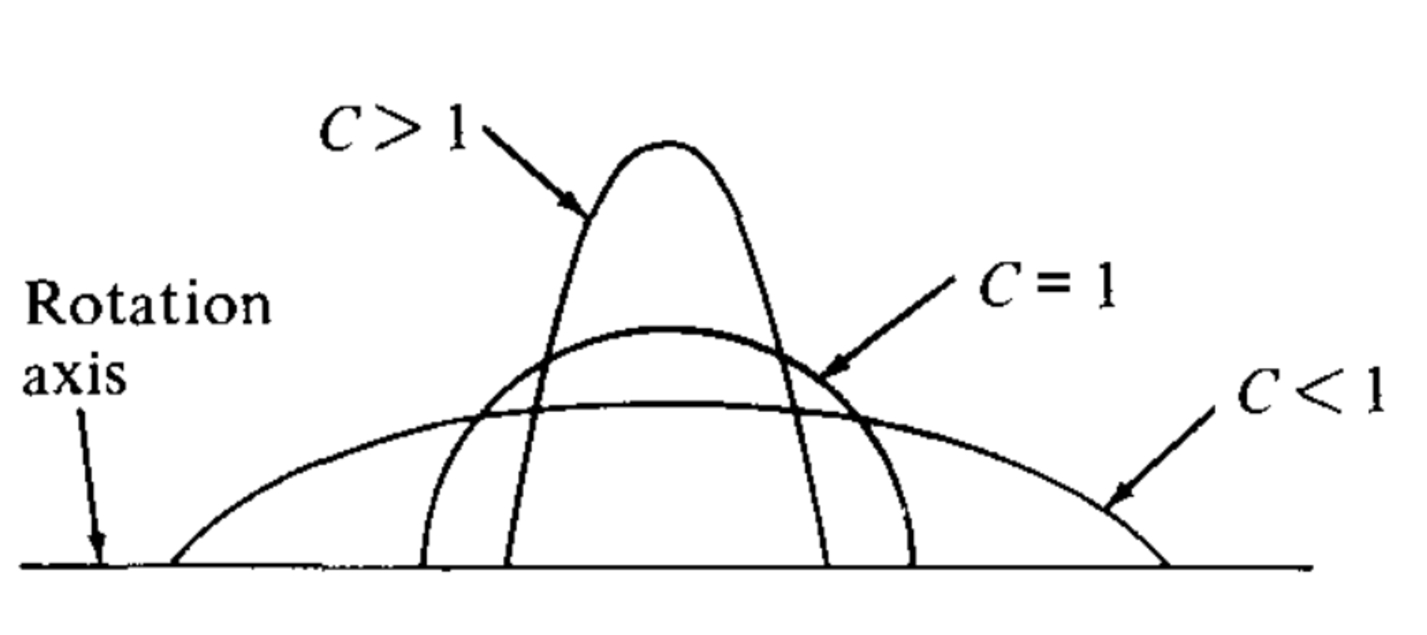
\includegraphics[scale=0.45]{3}
\caption{\textsc{The profile of the surface in the $xz$ plane for the cases $C=1,C>1,C<1$.}}
\end{figure}
\item \textit{All surfaces of revolution with constant curvature $K=-1$ may be given by one of the following types:}
\begin{enumerate}
\item $\varphi \left( v \right) = C\cosh v,\psi \left( v \right) = \int_0^v {\sqrt {1 - {C^2}{{\sinh }^2}v} dv} .$ 
\item $\varphi \left( v \right) = C\sinh v,\psi \left( v \right) = \int_0^v {\sqrt {1 - {C^2}{{\cosh }^2}v} dv} .$ 
\item $\varphi \left( v \right) = {e^v},\psi \left( v \right) = \int_0^v {\sqrt {1 - {e^{2v}}} dv} .$ 
\end{enumerate}
\textit{Determine the domain of $v$ and draw a rough sketch of the profile of the surface in the $xz$ plane.}
\item \textit{The surface of type c in part 3 is the pseudosphere of Exercise 6.}
\item \textit{The only surfaces of revolution with $K \equiv 0$ are the right circular cylinder, the right circular cone, and the plane.}
\end{enumerate}
\textsc{Solution.}
\begin{enumerate}
\item Let 
\begin{align}
\label{1.107}
\mathbf{x}\left( {u,v} \right) = \left( {\varphi \left( v \right)\cos u,\varphi \left( v \right)\sin u,\psi \left( v \right)} \right),\hspace{0.2cm} \varphi \left(v\right) \ne 0,
\end{align}
where the domain of $u$ and $v$ will be determined, be a parametrization of given surface, denoted by $S$ as usual, of revolution. We shall compute the Gaussian curvature of the points of surface $S$ by the parametrization \eqref{1.107}. To this end, we compute 
\begin{align}
{\mathbf{x}_u} &= \left( { - \varphi \left( v \right)\sin u,\varphi \left( v \right)\cos u,0} \right),\\
{\mathbf{x}_v} &= \left( {\varphi '\left( v \right)\cos u,\varphi '\left( v \right)\sin u,\psi '\left( v \right)} \right),\\
{\mathbf{x}_{uu}} &= \left( { - \varphi \left( v \right)\cos u, - \varphi \left( v \right)\sin u,0} \right),\\
{\mathbf{x}_{uv}} &= \left( { - \varphi '\left( v \right)\sin u,\varphi '\left( v \right)\cos u,0} \right),\\
{\mathbf{x}_{vv}} &= \left( {\varphi ''\left( v \right)\cos u,\varphi ''\left( v \right)\sin u,\psi ''\left( v \right)} \right),
\end{align} 
From these, we obtain the coefficients of the first fundamental form
\begin{align}
E &= \left\langle {{\mathbf{x}_u},{\mathbf{x}_u}} \right\rangle \\
 &= {\varphi ^2}\left( v \right){\sin ^2}u + {\varphi ^2}\left( v \right){\cos ^2}u\\
 &= {\varphi ^2}\left( v \right),\\
F &= \left\langle {{\mathbf{x}_u},{\mathbf{x}_v}} \right\rangle \\
 &=  - \varphi \left( v \right)\varphi '\left( v \right)\sin u\cos u + \varphi \left( v \right)\varphi '\left( v \right)\sin u\cos u\\
 &= 0,\\
G &= \left\langle {{\mathbf{x}_v},{\mathbf{x}_v}} \right\rangle \\
& = {\left( {\varphi '\left( v \right)} \right)^2}{\cos ^2}u + {\left( {\varphi '\left( v \right)} \right)^2}{\sin ^2}u + {\left( {\psi '\left( v \right)} \right)^2}\\
 &= {\left( {\varphi '\left( v \right)} \right)^2} + {\left( {\psi '\left( v \right)} \right)^2}\\
 &= 1,\mbox{ by the assumption \eqref{1.104}}.
\end{align}
Introducing the values just obtained in the coefficients of the second fundamental form gives
\begin{align}
e &= \left\langle {N,{\mathbf{x}_{uu}}} \right\rangle \\
 &= \frac{{\left( {{\mathbf{x}_u},{\mathbf{x}_v},{\mathbf{x}_{uu}}} \right)}}{{\sqrt {EG - {F^2}} }}\\
 &= \frac{{\left| {\begin{array}{*{20}{c}}
{ - \varphi \left( v \right)\sin u}&{\varphi '\left( v \right)\cos u}&{ - \varphi \left( v \right)\cos u}\\
{\varphi \left( v \right)\cos u}&{\varphi '\left( v \right)\sin u}&{ - \varphi \left( v \right)\sin u}\\
0&{\psi '\left( v \right)}&0
\end{array}} \right|}}{{\left| {\varphi \left( v \right)} \right|}}\\
 &=  - \psi '\left( v \right)\left| {\varphi \left( v \right)} \right|,\\
f &= \left\langle {N,{\mathbf{x}_{uv}}} \right\rangle \\
 &= \frac{{\left( {{\mathbf{x}_u},{\mathbf{x}_v},{\mathbf{x}_{uv}}} \right)}}{{\sqrt {EG - {F^2}} }}\\
 &= \frac{{\left| {\begin{array}{*{20}{c}}
{ - \varphi \left( v \right)\sin u}&{\varphi '\left( v \right)\cos u}&{ - \varphi '\left( v \right)\sin u}\\
{\varphi \left( v \right)\cos u}&{\varphi '\left( v \right)\sin u}&{\varphi '\left( v \right)\cos u}\\
0&{\psi '\left( v \right)}&0
\end{array}} \right|}}{{\left| {\varphi \left( v \right)} \right|}}\\
 &= 0,\\
g &= \left\langle {N,{\mathbf{x}_{vv}}} \right\rangle \\
& = \frac{{\left( {{\mathbf{x}_u},{\mathbf{x}_v},{\mathbf{x}_{vv}}} \right)}}{{\sqrt {EG - {F^2}} }}\\
& = \frac{{\left| {\begin{array}{*{20}{c}}
{ - \varphi \left( v \right)\sin u}&{\varphi '\left( v \right)\cos u}&{\varphi ''\left( v \right)\cos u}\\
{\varphi \left( v \right)\cos u}&{\varphi '\left( v \right)\sin u}&{\varphi ''\left( v \right)\sin u}\\
0&{\psi '\left( v \right)}&{\psi ''\left( v \right)}
\end{array}} \right|}}{{\left| {\varphi \left( v \right)} \right|}}\\
& = \frac{{\varphi \left( v \right)}}{{\left| {\varphi \left( v \right)} \right|}}\left( {\varphi ''\left( v \right)\psi '\left( v \right) - \varphi '\left( v \right)\psi ''\left( v \right)} \right).
\end{align}
Hence, the Gaussian curvature $K$ is given by
\begin{align}
K &= \frac{{eg - {f^2}}}{{EG - {F^2}}}\\
 &=  - \frac{{\psi '\left( v \right)\left| {\varphi \left( v \right)} \right| \cdot \frac{{\varphi \left( v \right)}}{{\left| {\varphi \left( v \right)} \right|}}\left( {\varphi ''\left( v \right)\psi '\left( v \right) - \varphi '\left( v \right)\psi ''\left( v \right)} \right)}}{{{\varphi ^2}\left( v \right)}}\\
& =  - \frac{{\psi '\left( v \right)\left( {\varphi ''\left( v \right)\psi '\left( v \right) - \varphi '\left( v \right)\psi ''\left( v \right)} \right)}}{{\varphi \left( v \right)}}.
\end{align}

It is convenient to put the Gaussian curvature in another form. By differentiating \eqref{1.104} we obtain
\begin{align}
\varphi '\left( v \right)\varphi ''\left( v \right) =  - \psi '\left( v \right)\psi ''\left( v \right).
\end{align} 
Thus, 
\begin{align}
K &=  - \frac{{\psi '\left( v \right)\left( {\varphi ''\left( v \right)\psi '\left( v \right) - \varphi '\left( v \right)\psi ''\left( v \right)} \right)}}{{\varphi \left( v \right)}}\\
 & =  - \frac{{\varphi ''\left( v \right){{\left( {\psi '\left( v \right)} \right)}^2} + \varphi ''\left( v \right){{\left( {\varphi '\left( v \right)} \right)}^2}}}{{\varphi \left( v \right)}}\\
& =  - \frac{{\varphi ''\left( v \right)}}{{\varphi \left( v \right)}}.
\end{align}
Thus, $\varphi$ satisfies the following equation
\begin{align}
\label{1.141}
\varphi '' + K\varphi  = 0,
\end{align}
and, by integrating the equation $\psi '\left( v \right) = \sqrt {1 - {{\left( {\varphi '\left( v \right)} \right)}^2}} $, $\psi$ is given by
\begin{align}
\label{1.142}
\psi  = \int {\sqrt {1 - {{\left( {\varphi '} \right)}^2}} dv} ,
\end{align}
Thus, $0<u<2\pi$ and the domain of $v$ is such that the last integral makes sense.
\item Plugging $K=1$ in \eqref{1.141} gives
\begin{align}
\varphi '' + \varphi =0 .
\end{align}
Solving this homogeneous second-order linear differential equation yields
\begin{align}
\label{1.144}
\varphi \left( v \right) = {C_1}\cos v + {C_2}\sin v,
\end{align}
where $C_1$ and $C_2$ are arbitrary constants.

Recall that the generating curve $\left(\varphi \left(v\right),\psi \left(v\right)\right)$ is in the $xOz$ plane and the surface of revolution $\mathbf{x}\left(u,v\right)$ is generated by rotating the generating curve around the $z$-axis. Since the surfaces of revolution intersects perpendicularly the plane $xOy$, the generating curves must intersects perpendicularly with the $x$-axis.

Assume that the generating curve $\left(\varphi \left(v\right),\psi \left(v\right)\right)$ intersects the $x$ axis at the point $\left(C,0\right)$ where $C =\varphi \left(0\right)$, since $\left(\varphi \left(v\right),\psi \left(v\right)\right)$ intersects the $x$-axis perpendicularly, the tangent vector of $\left(\varphi \left(v\right),\psi \left(v\right)\right)$ is perpendicular to the $x$-axis at the intersection $\left(C,0\right)$ (this also gives $\varphi \left(0\right)=C,\psi \left(0\right)=0$) , i.e.
\begin{align}
\varphi '\left( 0 \right) &= \left\langle {\left( {\varphi '\left( 0 \right),\psi '\left( 0 \right)} \right),\left( {1,0} \right)} \right\rangle \\
 &= 0.
\end{align}
Now, combining \eqref{1.144} with $\varphi \left(0\right) =C, \varphi '\left(0\right) =0$ yields ${C_1} = C,{C_2} = 0$, i.e. \eqref{1.144} becomes
\begin{align}
\label{1.147}
\varphi \left( v \right) = C\cos v.
\end{align}
And \eqref{1.142} then becomes, note that $\psi \left(0\right)=0$
\begin{align}
\label{1.148}
\psi \left( v \right) = \int_0^v {\sqrt {1 - {C^2}{{\sin }^2}\bar v} d\bar v} .
\end{align}
The domain of $v$ is, therefore, determined by requiring that the integrand in \eqref{1.148} makes sense, i.e., the domain of $v$ is given by
\begin{align}
\left\{ {v:0 < v < \pi ,\left| {\sin v} \right| \le \frac{1}{{\left| C \right|}}} \right\}.
\end{align}

In the case when $C=1$, \eqref{1.147}-\eqref{1.148} gives a sphere.
\item Plugging $K=-1$ in \eqref{1.141} gives 
\begin{align}
\varphi '' - \varphi =0.
\end{align}
Solving this homogeneous second-order linear differential equation gives 
\begin{align}
\label{1.155}
\varphi \left( v \right) = {C_1}{e^v} + {C_2}{e^{ - v}},
\end{align}
where $C_1$ and $C_2$ are arbitrary constants.

We consider the following three cases for the constants $C_1,C_2$.\footnote{Is it true that all surfaces of revolution with constant curvature $K=-1$ may be given by one of the given types?}
\begin{enumerate}
\item \textit{Case $C_1=C_2=\frac{C}{2}$.} In this case, \eqref{1.155} becomes
\begin{align}
\varphi \left( v \right)& = \frac{C}{2}\left( {{e^v} + {e^{ - v}}} \right)\\
& = C\cosh v,\\
\psi \left( v \right) &= \int_0^v {\sqrt {1 - {C^2}{{\sinh }^2}\bar v} d\bar v} .
\end{align}
where the domain of $v$ is chosen for which the last integral makes sense. 
\item \textit{Case $C_1 =\frac{C}{2},C_2=-\frac{C}{2}$.} In this case, \eqref{1.155} becomes
\begin{align}
\varphi \left( v \right) &= \frac{C}{2}\left( {{e^v} - {e^{ - v}}} \right)\\
 &= C\sinh v,\\
\psi \left( v \right) &= \int_0^v {\sqrt {1 - {C^2}{{\cosh }^2}\bar v} d\bar v} .
\end{align}
where the domain of $v$ is chosen for which the last integral makes sense. 
\item \textit{Case $C_1=1,C_2=0$.} In this case, \eqref{1.155} becomes
\begin{align}
\varphi \left( v \right) &= {e^v},\\
\psi \left( v \right) &= \int_0^v {\sqrt {1 - {e^{2\bar v}}} d\bar v} .
\end{align} 
where the domain of $v$ is chosen for which the last integral makes sense. 
\end{enumerate}
\item We claim that the surface of type 3 in $\left(3\right)$ is the pseudosphere described in Problem 1. To this end, we check the following generating curve
\begin{align}
\label{1.156}
\varphi \left( v \right) = {e^v},\psi \left( v \right) = \int_0^v {\sqrt {1 - {e^{2\bar v}}} d\bar v} ,
\end{align}
is the tractrix. We turn back to equation \eqref{1.43}, but now we set $x=e^v$ instead of setting $x= \sin \theta$ as before. Then integrating \eqref{1.43} with respect to $v$ yields 
\begin{align}
z &= \int {\frac{{\sqrt {1 - {e^{2v}}} }}{{{e^v}}}{e^v}dv} \\
& = \int {\sqrt {1 - {e^{2v}}} dv} .
\end{align}
Hence, \eqref{1.156} yields a parametrization for the tractrix. Finally, since the tractrix is the generating curve for the pseudosphere, the surface 
\begin{align}
\left( {{e^v}\cos u,{e^v}\sin u,\int_0^v {\sqrt {1 - {e^{2\bar v}}} d\bar v} } \right),
\end{align}
with suitable domains of $u$ and $v$, is exactly the pseudosphere.
\item Plugging $K=0$ in \eqref{1.141} yields $\varphi '' =0$. Hence, 
\begin{align}
\varphi \left( v \right) = {C_1}v + {C_2},
\end{align}
where $C_1$ and $C_2$ are arbitrary constants. Plugging $\varphi '\left(v\right) = C_1$ in \eqref{1.142} gives
\begin{align}
\psi \left( v \right) &= \int_0^v {\sqrt {1 - C_1^2} d\bar v} \\
 &= v\sqrt {1 - C_1^2} ,
\end{align}
where $-1\le C_1\le 1$. 

We consider the following three cases with respect to $C_1$.
\begin{enumerate}
\item \textit{Case $\left| {{C_1}} \right| = 1$.} In this case, the generating curve becomes 
\begin{align}
\left( {\varphi \left( v \right),\psi \left( v \right)} \right) = \left( { \pm v + {C_2},0} \right),
\end{align}
which is a line orthogonal to the $z$-axis.
\item \textit{Case $C_1 =0$.} In this case, the generating curve becomes
\begin{align}
\left( {\varphi \left( v \right),\psi \left( v \right)} \right) = \left( {{C_2},v} \right),
\end{align}
which is a line orthogonal to the $x$-axis. Therefore, the surface of revolution in this case is a right circular cylinder.
\item \textit{Case $0 < \left| {{C_1}} \right| < 1$.} In this case, the generating curve becomes
\begin{align}
\left( {\varphi \left( v \right),\psi \left( v \right)} \right) = \left( {{C_1}v + {C_2},v\sqrt {1 - C_1^2} } \right),
\end{align}
which is a line intersecting the $z$-axis. Therefore, the surface of revolution in this case is a right circular cone. \hfill $\square$
\end{enumerate}
\end{enumerate}
\vspace{1cm}
\begin{center}
\textsc{The End}
\end{center}
\newpage
\begin{thebibliography}{999}
\bibitem {1} Manfredo P. do Carmo, \textit{Differential Geometry of Curves and Surfaces}, 1st edition,  Prentice-Hall, Inc., Englewood Cliffs, New Jersey. 1976.
\bibitem {2} Wolfgang K\"{u}hnel, \textit{Differential Geometry, Curves – Surfaces – Manifolds}, Second Edition, Student Mathematical Library, Volume 16, AMS.
\bibitem {3} \url{http://mathworld.wolfram.com/Pseudosphere.html}
\end{thebibliography}
\end{document}